%%%%%%%%%%%%%%%%%%%%%%%%%%%%%%%%%%%%%%%%%%%%%%%%%%%%%%%%%%%%%%%%%%%
%                                                                 %
%                            CHAPTER ONE                          %
%                                                                 %
%%%%%%%%%%%%%%%%%%%%%%%%%%%%%%%%%%%%%%%%%%%%%%%%%%%%%%%%%%%%%%%%%%%

\chapter{INTRODUCTION}

\section{Introduction}

\begin{quotation}
	If scientific data production were easy, instruments would
	have stable calibrations and validation activities would discover no need for
	corrections that vary with time. Unfortunately, validation invariably shows that
	instrument calibrations drift and that algorithms need a better physical basis.
\end{quotation} \cite{Barkstrom2003}.

Anyone who has used an iPhone or owned a video game console understands the basics of versioning.
Companies brand sequential devices to indicate improvements in performance or capabilities.
This basic identification method has given rise to a plethora of versioning systems used widely across a landscape of software and data.
They help scientific workflows avoid losing work by managing transitions and changes while in operation \cite{Casati1996}.
They provide necessary documentation which informs the transition to new methods and procedures \cite{Wiil:2000:RDH:338407.338517}.
They provide accountability for the value of a project's data set when considering an agency's continued funding \cite{Cavanaugh2002}.
The natural evolution of these systems, however, have given rise to formal architecture operating on top of very informal concepts.
In this dissertation, we identify gaps in versioning practices which result from tradition and develop a data model to more completely capture the interactions involved in versioning.

\section{Definitions of Version}

Using versions in the vernacular has become so pervasive that few documents formally define it.
Barkstrom describes versions as \textbf{homogeneous groupings} used to control, ``production volatility induced by changes in algorithms and coefficients as result of validation and reprocessing," \cite{Barkstrom2003}.
The \textbf{groupings} he mentions is a method of separating data objects such that they have similar scientific or technical properties.
In order to determine when these properties have changed, he leverages the NASA workflow model shown in Figure \ref{NASALevels}.
\begin{figure}
	\centering
	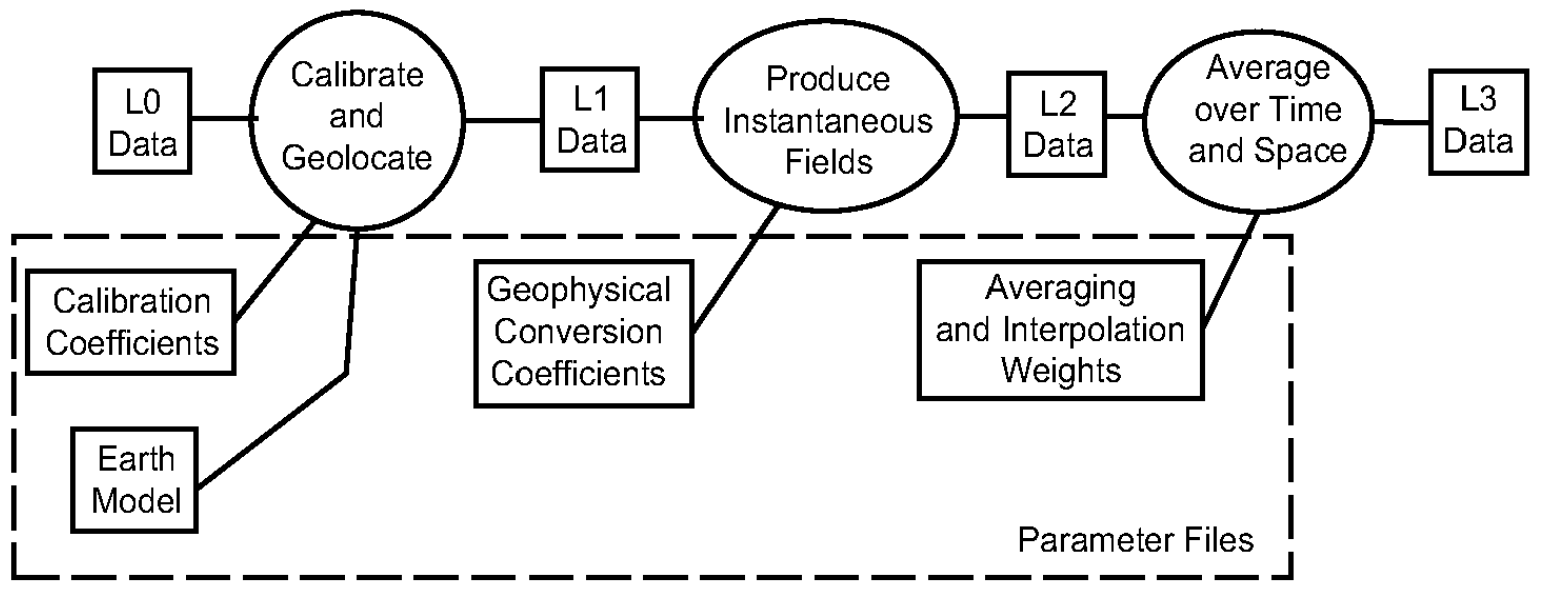
\includegraphics[scale=0.35]{figures/NASALevels.png}
	\caption[NASA organizes its data into three levels depending on the amount of aggregation and the distance the data is removed from the original sensor measurements.]{NASA organizes its data into three levels depending on the amount of aggregation and the distance the data is removed from the original sensor measurements. Figure 1 from \cite{Barkstrom2003}}
	\label{NASALevels}
\end{figure}
The model describes the formal stages of processing to turn a raw remote sensing signal from satellite instruments into global aggregate summaries \cite{Barkstrom2003}.
Understanding this model reveals that changes to either the algorithms or parameter files will force a change in the resulting data, creating a new version of the output data.
Essentially, versions are a means to communicate how much data has diverged as a result of changes to an object's provenance.

Another definition comes from Tagger in which versions are a, ``semantically meaningful snapshot of a design object," \cite{Tagger2005}.
He, unfortunately, does not further clarify what he means by semantically meaningful.
The design object unifies the versions as their primary subject, capturing the object's state over the course of its design.

The derivation, PROV Ontology's analog for a version and covered more in Section \ref{sec:prov}, is defined as, ``a transformation of an entity into another, an update of an entity resulting in a new one, or the construction of a new entity based on a pre-existing entity," \cite{Lebo2013}.
In this view, a \textbf{version} exists in comparison to another object.

The Functional Requirements for Bibliographical Records (FRBR) avoids the terms \textbf{edition} and \textbf{version} since ``those terms are neither clearly defined nor uniformly applied" \cite{frbr}.
Instead, they use the terms: work, expression, and manifestation.
A \textbf{work} refers to the abstract concept of a creative or artistic idea.
\textbf{Expressions} are then different forms of that particular \textbf{work}, embodying the most similar term to versions.
A \textbf{manifestation} is the physical embodiment of an \textbf{expression}.
These three terms and their hierarchy establish a repeating theme throughout other versioning works.
Combining these myriad of definitions together, a version is an \textbf{expression} of a \textbf{work} which exists in comparison to another object and communicates the extent to which it diverges from that object as a result of provenance changes.

\section{Version Systems} \label{sec:system}

Versioning systems take many different forms from Clotho, an application conducting versioning at the block level, to Champagne, a framework to propagate change data across multiple information systems \cite{Flouris04clotho:transparent} \cite{Systems02champagne:data}.
Each approach has a unique set of challenges to overcome.
Closer to the data collection, version systems must be flexible and responsive to adapt to changing environments, but as the socio-technical distance of a repository increases away from the collection site, more formal methods are required to unify repositories \cite{Baker2009}.
Different approaches are also necessary to account for the needs of different domains.
Versioning an XML text-file will need to account for serial file input and output as well as structured markup \cite{Chien:2000:VMX:646544.696357}.
Many applications have adopted a tree-like structure which is further propagated by software versioning managers (SVM) \cite{Stuckenholz:2005:CEV:1039174.1039197}.
The advantage being well established graph theory methods can be applied to complex objects relationships in complex environemtns \cite{Dijkstra1994}.
The growing population of web documents, however, presents a new smörgåsbord of complicated data which will need scalable solutions \cite{Berberich:2007:TMT:1277741.1277831}.

\subsection{Library Sciences}

While many of the modern systems requiring versioning managers store digital products, libraries have been tackling similar issues for a much longer time.
Libraries curate multiple editions of the same work, sometimes with significant revisions \cite{Wiil:2000:RDH:338407.338517}.
In many ways, versioned objects resemble multi-edition books or documents.
Digital librarians have faced many challenges when searching for a persistent identifier due to evolving web technologies.
Early citations referred to on-line documents using stagnant Uniform Resource Locators (URL), but this frequently lead to a condition known as link rot where moving the document would invalidate the URL \cite{Lyons2005}.
Locators required a system to manage changes of old identifiers to new locations when people attempted to utilize references from print.
The need eventually led to the development of Persistent URLs (PURL), which also suffered from link rot, and this eventually led to the distributed Digital Object Identifier (DOI) system used to track documents today \cite{Duerr2011}.
The PURL used a centralized system that would translate dead links and redirect to a document's latest location.
The system would still need to be manually updated, meaning links would rot if a document was lost or overlooked.
DOIs rely on a network of managing agencies to collect and host submitted documents.
In the specialized Handle system, the network has member agencies internally assign an unique name and concatenate it to the end of their host name.
In Figure \ref{table:Duerr}, DOIs represent the most suitable identifier used for citation in scholarly literature \cite{Duerr2011}.
\begin{figure}
	\centering
	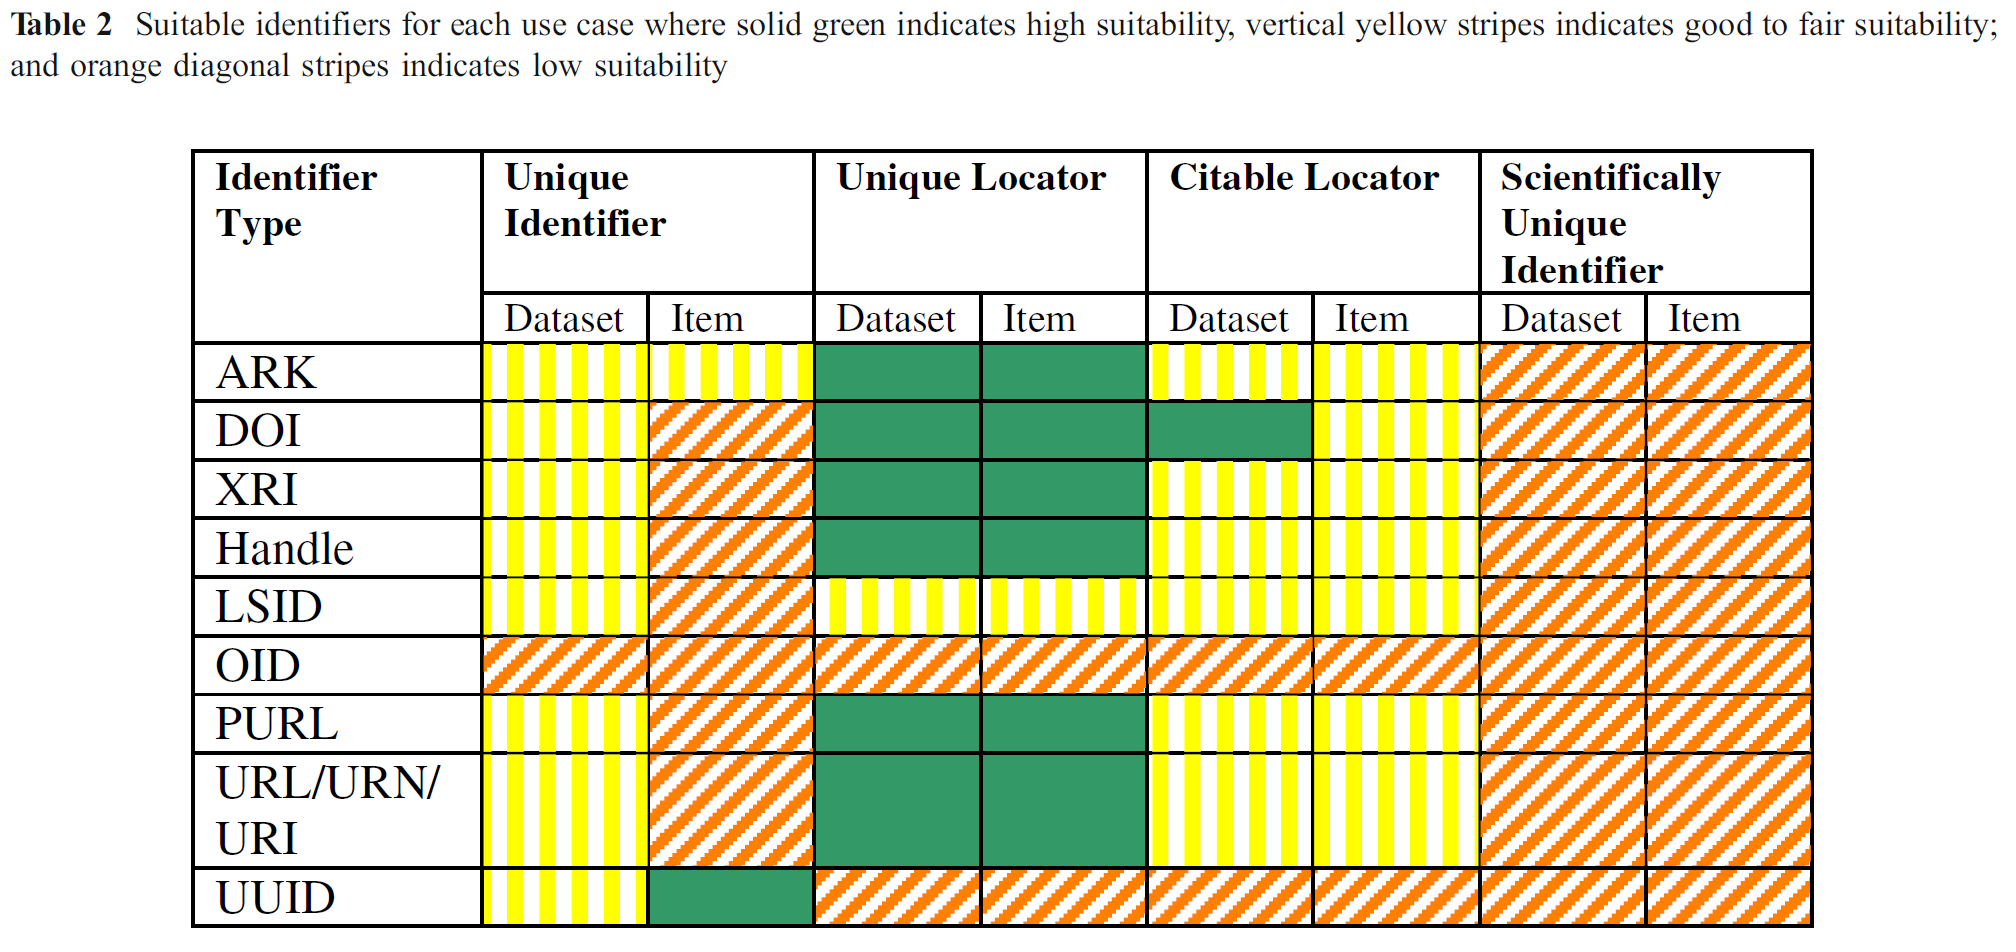
\includegraphics[scale=0.30]{figures/DigitalIdentifierTable.png}
	\caption[Table of predominant identifiers used in science.]{Table of predominant identifiers used in science.  From Duerr, et al. \cite{Duerr2011}}
	\label{table:Duerr}
\end{figure}
The DOI network provides a robust system to track documents, but when tracking data, it faces difficulty following the rate of change with more volatile data sets.
Under current definitions, distribution organizations assign different DOIs to separate editions of a document.
Documents often do not need new identifiers since they change very rarely as a result of the publication process.
Data set production and distribution cycles move more quickly and react more sensitively to small content changes, including when data collection continues on after initial publication.
Data set behavior becomes entirely too slow as data providers begin allowing users to dynamically generate data products from existing data according to their needs \cite{Barkstrom2003a}.
Some agencies have begun assigning versioned DOIs, but this has not become common practice.
Other groups do not assign a new DOI, but reference the latest release of the document or object \cite{Ands2017}.

As digital methods have evolved, so have digital libraries.
The documents that digital libraries store are no longer constrained by physical organization \cite{Barkstrom_digitallibrary}.
A book can physically be randomly stored for efficient retrieval, but the digital copy may reside in multiple locations depending on dynamic filters or search queries.
The Mellon Fedora Project developed a standardized edition control structure to unify disparate digital library stores \cite{Payette2002}.
The regularizing edition tracking methods significantly improved the response time and relevancy of the library services.

\subsection{Software Versioning}

Software versions form the most visible displays of versioning often experienced by researchers.
Version managers provide tools to archive and restore code through the development lifecycle.
The Revision Control System (RCS), developed in originally in 1985, documents one of the earliest uses of the dot-decimal identifier \cite{tichy1985rcs}.
This identifier uses a sequence of whole numbers concatenated by decimals.
The system possessed many features of modern SVMs such as branches, a separate copy of the code for developing changes safely, which were identified by extending the dot-decimal identifier as seen in Figure \ref{RCSTree}.
\begin{figure}
	\centering
	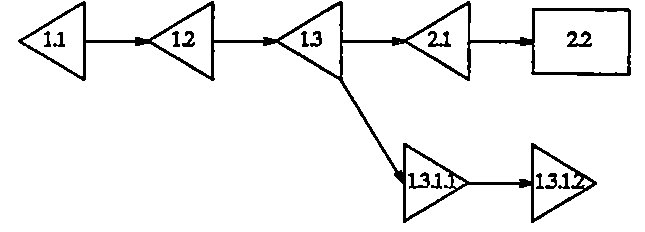
\includegraphics[scale=0.75]{figures/RCSCommitTree.png}
	\caption[Commit history of an object in RCS with changes in the main line stored as back deltas and side branches stored as forward deltas.]{Commit history of an object in RCS with changes in the main line stored as back deltas and side branches stored as forward deltas.  Figure 5 in \cite{tichy1985rcs}}
	\label{RCSTree}
\end{figure}
Not long after, the Concurrent Versions System (CVS) gained popularity with methods allowing multiple users to concurrently develop code to a central repository \cite{cederqvist2002version}.
The most popular modern SVM is GIT which also allows concurrent development but enables distributed repositories \cite{Chacon:2009:PG:1618548}.
Each developer contributing to a project is considered by the system to possess the master copy of that project.
The users collaborate by requesting and pulling other developer's master copies into their project.
In previous SVMs, only the differences between software files were stored, but GIT stores the entirety of each file version.
Figure \ref{GITFile} demonstrates an example of how GIT employs storage space for multiple versions \cite{Chacon:2009:PG:1618548}.
\begin{figure}
	\centering
	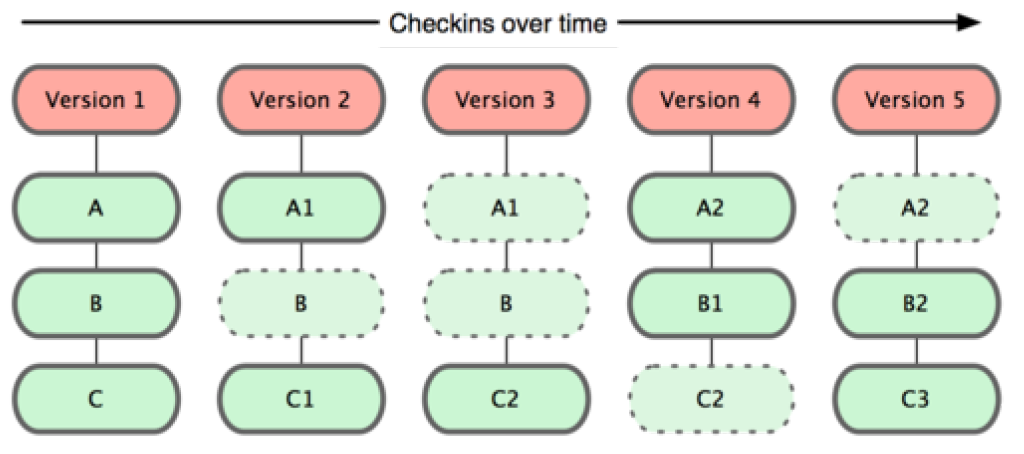
\includegraphics[scale=0.50]{figures/GITFiles.png}
	\caption[GIT stores changes in the repository as snapshots of individual files.]{GIT stores changes in the repository as snapshots of individual files. Figure 1.5 from \cite{Chacon:2009:PG:1618548}}
	\label{GITFile}
\end{figure}
Only a pointer is stored in subsequent versions for unchanged files, saving space.
Fischer, et al., demonstrate the importance of software version systems by integrating the manager with a bug tracking system to indicate the bugs a version release addresses \cite{Fischer2003}.

\subsection{Database Versioning}

The need for dta versioning methods grew alongside the growing popularity and power of relational databases.
Klahold, et al., introduced using abstract versioning environments in 1986 to separate the temporal features and organize the data into related groupings \cite{Klahold:1986:GMV:645913.671314}.
Research in the versioning area focused primarily on the database schema.
The results were temporal databases where schemas included time and dated transactions modifying the schema \cite{roddick1996model}.
Temporal databases allowed old queries to be executed on updated schemas, improving the reproducibility of results.
Capturing periodic snapshots or copies becomes unfeasible with increasingly large centralized database systems.
Data collection continues to migrate towards massive data warehouses which store and serve a wide variety of data \cite{Vassiliadis1999}.
Proell and Rauber have investigated tracking data queries instead of the database as a more scalable solution to reproduce data \cite{proellBigData}.
The queries can then be used as publication citations to provide scalable, reproducible references to older data \cite{Proell2013} \cite{DBLP:conf/data/2013}.

\subsection{Grid Versioning}

The grid provides a sensitive environment for versioning where there are many users and data movement across the grid should be avoided.
The CERN grid for the Compact Muon Solenoid experiment carefully developed processes which allow references by multiple users to the same file without copying that file across the grid \cite{Holtman:687353}.
Versions lock and release to permit parallel processing while still archiving additions and modifications to the data.
Grid versioning applications also begins to highlight the difference in versioning usage patterns between users and producers \cite{Branco2008}.
Deeper exploration into the ATLAS system documentation did not reveal specific use cases explaining the differences.
The grid also provides users with the ability to begin dynamically defining data sets to their needs by aggregating results from across the network \cite{Barkstrom2003a}.
The process would create new data sets without prior existing change documentation and fueled a demand for responsive frameworks which could track the discordant data collection conditions assimilated by the system \cite{Kovse2003VGridAVS}.

\subsection{Ontology Versioning}

Ontologies play a major role in defining domains, especially in the biological and medical fields where terms and definitions can change rapidly across highly variable organisms \cite{Ochs:2015:SVS:2826733.2826866}.
As a result, the ontologies require consistent methods to capture and model changes to evolving terms.
Tools aid in the process by detecting differences between ontologies \cite{Hartung201315}.
Klein and Fensel have found that when the changes are discovered, both forward and backward compatibility must be established for clear ontology versioning \cite{Klein01ontologyversioning}.
Not only must the path from an old term to a new one be clear, but a method for new terms to interact with old data must also exist.
They additionally identified three levels at which ontologies can differ: the domain, the conceptualization, and the specification.
Hauptmann et al., define a method to version ontologies natively within a triple store using linked data \cite{HauptmannEtAl:LDQ2015} \cite{LDQ2015}.
The method heavily relies on the context of stored data.


\section{Version Models} \label{sec:models}

Version models provide a visual a theoretical aid in understanding where a data object lies in relation to the rest of a work.
The Atmospheric Radiation Measurements (ARM) group used a model dividing the data into mathematical sets which versioning operations acted upon\cite{6906868}.
Adding files already in the set created a new set which inherited all non-intersecting files and included all the new ones.
The model provided a means to organize and automate the versioning of ARM's daily expanding data sets.

The Health Care and Life Sciences (HCLS) Interest Group of the World Wide Web Consortium (W3C) recently released a model which may provide a solution when used in conjunction with other identifiers \cite{Dummontier2016}.
Their model, shown in Figure \ref{HCLSModel}, separates the concept of a data set into three groupings.
\begin{figure}%[b]
	\centering
	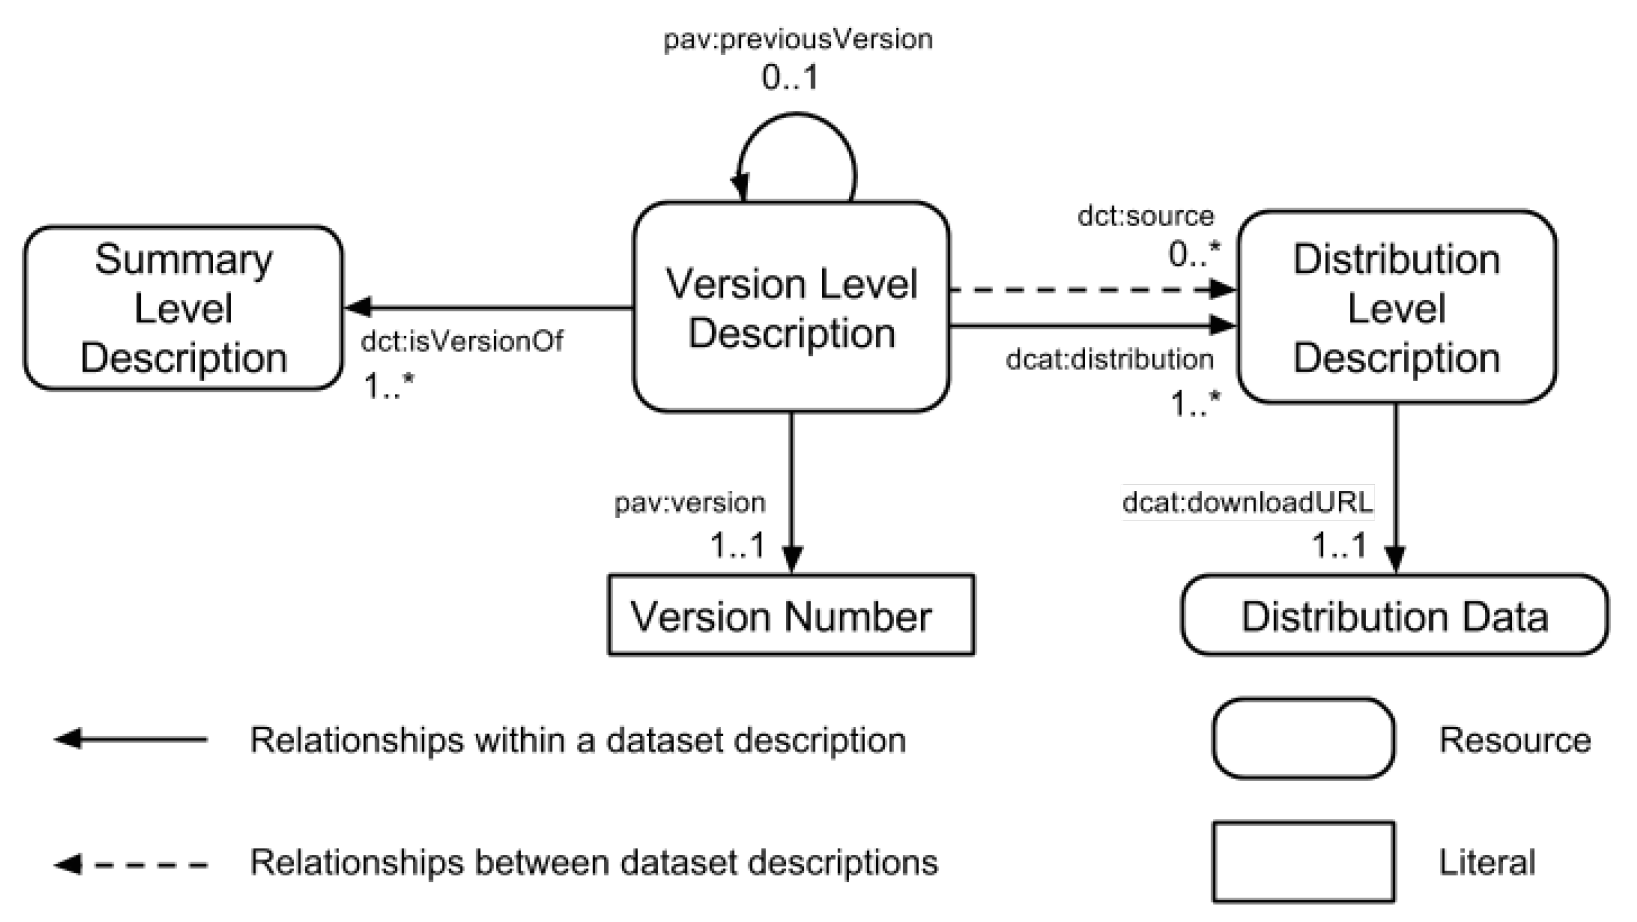
\includegraphics[scale=0.35]{figures/HCLSModel.png}
	\caption[Data model from the Health Care and Life Sciences Interest Group separating data into three levels: works, versions, and instances.]{Data model from the Health Care and Life Sciences Interest Group separating data into three levels: works, versions, and instances.  From Dummontier, et al. \cite{Dummontier2016}}
	\label{HCLSModel}
\end{figure}
The highest level summarizes the data as an abstract work, perhaps better described as a topic or title.
The data topic can have multiple versions over time.
The version can then be instantiated into various distributions with different physical formats.
The model---relating summary, version, and distribution---also strongly resembles the formation of FRBR's work, expression, and manifestation model.

\begin{figure}
	\centering
	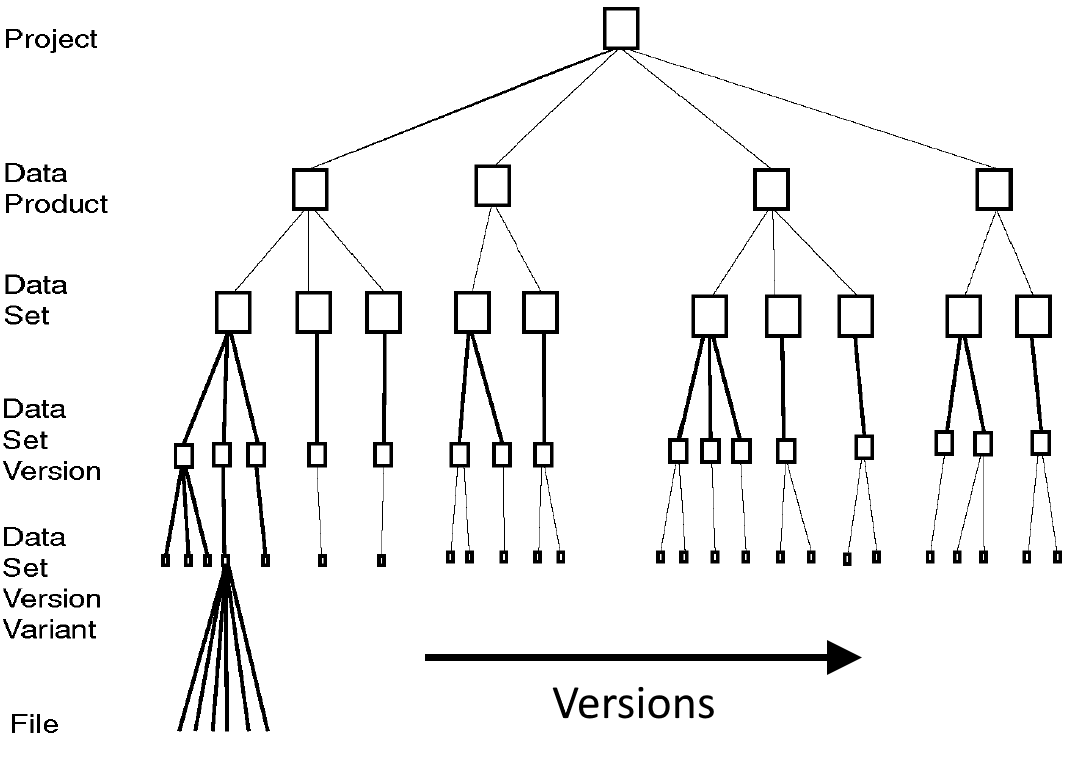
\includegraphics[scale=0.50]{figures/hierarchy.png}
	\caption[Visual representation of grouping hierarchy.]{Visual representation of grouping hierarchy.  From \cite{Barkstrom2003}}
	\label{hierarchy}
\end{figure}

From his definition of versions, Barkstrom also outlines an hierarchical version model as seen in Figure \ref{hierarchy}.
The model features additional intermediary levels than the HCLS's model, following NASA's data curation practices \cite{barkstrom2014earth}.
Each edge in the tree signifies a difference with other objects at the same depth, but the model does not provide a mechanism to explain the difference.

\section{Provenance Ontologies}

Provenance ontologies form a major section of linked data approaches to data versioning.
The coverage stems from the close relation between provenance and differentiating versions.
The Proof Markup Language, one of the first semantic models to capture provenance information, expressed lineage relationships using inference reasoning through traceable graphs \cite{daSilva2006381}.
The technique provides a powerful way to express and imply sequences of relationships between different versions and characterize the manner of their relation.

\subsection{Open Provenance Model}

A number of linked data models include versioning concepts such as the Open Provenance Model (OPM) \cite{moreau2008open}.
Driven by the uncertain needs and sometimes conflicting conventions of different scientific domains, the model sought to find a method to standardize the way in which provenance data is captured while also keeping the specification open to accommodate current data sets through the change.
In an experimental case, the model has been applied to sensor networks, automating and unifying their provenance capture even as they grow \cite{5478496}.
To aid OPM's adoption, the framework Karma2 integrates provenance capture into scientific workflows and provides a more abstract view of their data collection activities \cite{simmhan2010karma2}.
The property \textit{opm:WasDerivedFrom} constitutes a core concept in the model and marks the reliance of one object's existence on another object.
For a large part, this encompasses the engagement which provenance models view versions, without further need to explore the derivation's content.

\subsection{PROV-O}\label{sec:prov}

PROV, a World Wide Web Consortium (W3C) Recommendation, delineates a method to express data provenance in a more compact form as seen in Figure \ref{PROVO} \cite{Gil2013a} \cite{Groth2013}.
\begin{figure}
	\centering
	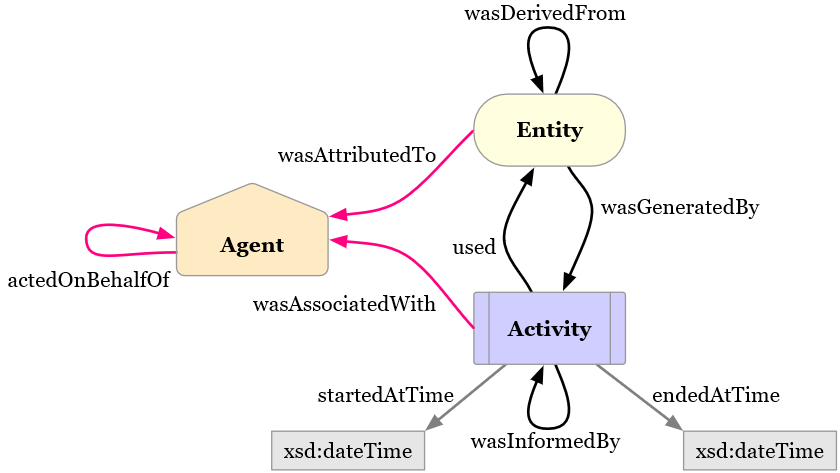
\includegraphics[scale=0.5]{figures/ProvO.png}
	\caption[Diagram of the PROV Ontology.]{Diagram of the PROV Ontology.  Figure 1 from \cite{Lebo2013}}
	\label{PROVO}
\end{figure}
The recommendation uses a conceptual model relating activities, agents, and entities to describe data production lineage \cite{Moreau2013c} \cite{Nies2013} \cite{Nies2013a}.
Intended as a high level abstraction, it takes an activity-oriented approach to provenance modeling.
Every data entity results from the actions of some activity \cite{Gil2013}.
The conceptual model's expression occurs through the PROV Ontology (PROV-O), which can be conveyed through various resource description languages \cite{Hua2013} \cite{Klyne2013}.
The ontology is further formalized into a functional notation for easier human consumption \cite{Moreau2013b} \cite{Cheney2013a}.
One particular strength that has contributed to the adoption of PROV is its ability to link into other ontologies, making it easier for existing semantically enriched data sets to adopt PROV \cite{Miles2013} \cite{Moreau2013}.

PROV has provided a major contribution in maintaining the quality and reproducibility of data sets and reporting in the National Climate Assessment (NCA) \cite{Ma2014191}.
The contribution signifies that there is an increased likelihood of adoption through other scientific fields as a result of this reporting.
The Global Change Information System, which houses the data used to generate the NCA, uses PROV to meticulously track the generation of its artifacts and results as they are used in assessment report \cite{Tilmes2012}.
The usage means that not only does the data have a traceable lineage to verify quality, but the content of documents can have the same verifiability \cite{Ma2014}.
Komadu, a framework developed to alleviate workflow integration, utilizes PROV to improve upon its predecessor, Karma, by no longer utilizing global context identifiers that were not necessarily shared throughout the workflow. \cite{Suriarachchi_2015}.

The PROV Ontology provides three different concepts that begin to encapsulate the provenance relationship between data versions.
It defines a \textit{prov:Generation} as "the completion of production of a new entity by an activity," \cite{Lebo2013}.
This means that the generation, which corresponds adding an object to a version, must result from a \textit{prov:Activity}.
\textit{Prov:Invalidation}, defined as the, ``start of the destruction, cessation, or expiry of an existing entity by an activity," makes a similar connection between activities and entities \cite{Lebo2013}.
A third concept, \textit{prov:Derivation}, relates two entities, and the ontology defines it as, "a transformation of an entity into another, an update of an entity resulting in a new one, or the construction of a new entity based on a preexisting entity. " \cite{Lebo2013}.
PROV also has a property called \textit{prov:isDerivedFrom} which conveys the same definition as a \textit{prov:Derivation}.
Using the property and concept together forms a qualified property which can be instantiated and further annotated.

\subsection{Provenance, Authorship, and Versioning Ontology}

The Provenance, Authorship, and Versioning (PAV) Ontology is, ``a lightweight vocabulary, for capturing ``just enough" descriptions essential for web resources representing digitized knowledge" \cite{Ciccarese2013}.
It provides a means to track versioning information through linked data by introducing \textit{pav:version} to cite versions and \textit{pav:previousVersion} to link them together in order \cite{Ciccarese2013}.
It does so in comparison to the Dublin Core concept \textit{dc:isVersionOf} which records, "Changes in version imply substantive changes in content rather than differences in format" \cite{DCMI2012}.
PAV supports the idea that a new concept becomes necessary to cover cases where new versions do not have to be substantive but can still be alternate editions of the original object.
While it documents related versions well, PAV does not dive deeper in explaining the circumstances behind version differences.

\subsection{Schema.org}

The Schema.org ontology is not a provenance ontology but provides a means to supply searchable web pages with standardized micro-data.
The ontology has a collection of concepts which could be applied to versioning.
The \textit{schema:UpdateAction} is defined as, ``the act of managing by changing/editing the state of the object," which encompasses the same responsibilities expected of versioning systems \cite{Schema}.
The terms \textit{schema:AddAction}, \textit{schema:DeleteAction}, and \textit{schema:ReplaceAction} subclass the \textit{shcema:UpdateAction}.
These classes model actions which further cement parallels between versioning and \textit{schema:UpdateAction}.

Schema.org defines a \textit{schema:ReplaceAction} as, ``the act of editing a recipient by replacing an old object with a new object" \cite{SchemaRep}.
The concept has two properties, \textit{schema:replacee} and \textit{schema:replacer} which indicates that a new object replaces an old one.
Schema.org models the interaction by placing the replacement action at the relation's center.
In comparison, the \textit{schema:AddAction} is defined as, ``the act of editing by adding an object to a collection" \cite{SchemaAdd}.
The action only involves the object and the new state of the collection, not involving any of the collection's prior lineage.
Schema.org defines the \textit{schema:DeleteAction} as, "the act of editing a recipient by removing one of its objects," \cite{SchemaRem}.
The concept aligns well with other versioning systems, although deletion may be a strong assertion.

\section{Change Logs} \label{sec:changelog}

Change logs, artifacts resulting from the versioning process, play a major role filling in gaps between versions.
The logs document changes and explain, in human language, motivations behind the modifications \cite{uel1037}.
Since identifiers denote that a change has occurred, the logs provide details on how the changes modify an object's attributes.
They demonstrate a need and utility in understanding the deeper content of change beyond knowing that an object did transform.
While some data sets will provide a change log, software projects have normalized their use in version release documentation.
As a result, these projects provide a basis for understanding the value these logs can supply data sets with multiple versions.
The change log's common drawback is the limitation to only human readable text.
Wider adoption among data sets may be possible by making these texts machine computable.

Open source projects use change logs more consistently than data projects, which usually sport only use documentation.
Logs play an important communication role in these projects since developers can contribute without having been part of the original development team.
The change logs allow developers to link bugs and errors with their corrections in new versions of the code \cite{Chen:2004:OCL:990374.990391}.
The links gives insight into motivations behind particular design decisions.
Logs linked with version releases also provide feedback to the user community that corrections have been addressed, in addition to ensuring that improvements drive modifications to the code base.
An identifier cannot communicate these qualities while remaining succinct.
Some research has been done to determine the health of a development project based on the number and length of change logs released over time \cite{German03automatingthe}.
Little work has been done to make change logs machine-computable, as many of these documents remain in human-readable text only.
Research done involving change log content must manually link entries with computable meta-data such as the introduction of new features with the emergence of new bugs \cite{6132954}.
While machines may still be significantly removed from the ability to comprehend the impact of changes made to a data set or software code, they are currently opaquely blocked from consuming any of the content within logs more than understanding they contain text.
The transition between different versions of large data sets is then left largely up to the human user's ability to understand and process the modifications mentioned within the change log.

\section{Introduction of Use Cases}

\subsection{Use Case 1: Linked Data Change Log}
The first use case's goal is to determine the differences between two versions of a data set.
The way this is accomplished in the ``Global Database on \textsuperscript{3}He/\textsuperscript{4}He in on-shore free-circulated subsurface fluids" (Noble Gas) is to look at the use documentation for each version and manually determine the differences \cite{Polyak2015}.
The ``Paragenetic Mode for Copper Minerals" (Copper) database became available through collaboration with the author's lab to create new methods of visualizing mineralogy relationships \cite{Morrison2016}.
In the Copper data set, changes were reported by word of mouth through interaction with the author.
These data sets were chosen because they had at least two versions in the same format, Excel spreadsheets.
Software projects normally use a change log to summarize the modifications separating two versions, but a document was not included with either data set.

The spreadsheets offered a very enticing point of entry since changes could easily be detected by comparing matching cells in a regular table format and tools to access the data were readily available.
Both data sets displayed content and structural changes, new or deleted rows and columns as well as re-ordered columns in the Copper data set's case.
Each version of the spreadsheets were also instanced, allowing multiple versions to simultaneously exist.
Separate linked data identifiers can then be assigned to each file, making graph generation possible.
Centralized databases were avoided because they generally only make available a single instance, causing manual verification and visual comparisons difficult.
In addition, users of centralized databases primarily interact with the data through queries, merging and filtering data tables to slice out the desired data set.
Rather than complicate the approach with multiple tables, Use Case 1 focuses on the primary unified table of the Noble Gas and Copper data sets.

The spreadsheets do not innately use linked data identifiers, meaning artificial identifiers will need to be deployed referring to objects within the model.
Methods to generate an identifier lies outside the scope of this work.

\subsection{Use Case 2: Change Distance}

\section{Hypothesis Statement}

Large data collection endeavors necessitate the development and deployment of versioning systems to manage change propagating through their data.
Advancing beyond identifier comparisons and delving into capturing substantive change can significantly improve the ability to standardize version communications and transition.
The work in the following chapters will contribute to expanding change capture by defining a more expressive linked data versioning model.
The model will allow current versioning documentation to become machine-consumable.
A better method will be developed to provide a quantitative basis for the assignment of version identifiers.

\section{Contributions}


%%% Local Variables:
%%% mode: latex
%%% TeX-master: t
%%% End:
